\subsection{Gridalt - Alternate Grid Package}
\label{sec:pkg:gridalt}
\begin{rawhtml}
<!-- CMIREDIR:package_gridalt: -->
\end{rawhtml}

\subsubsection {Introduction} 

The gridalt package is designed to allow different components of MITgcm to
be run using horizontal and/or vertical grids which are different from the main 
model grid. The gridalt routines handle the definition of the all the various
alternative grid(s) and the mappings between them and the MITgcm grid.
The implementation of the gridalt package which allows the high end atmospheric 
physics (fizhi) to be run on a high resolution and quasi terrain-following vertical 
grid is documented here.  The package has also (with some user modifications) been used 
for other calculations within the GCM. 

The rationale for implementing the atmospheric physics on a high resolution vertical
grid involves the fact that the MITgcm $p^*$ (or any pressure-type) coordinate cannot 
maintain the vertical resolution near the surface as the bottom topography rises above
sea level. The vertical length scales near the ground are small and can vary 
on small time scales, and the vertical grid must be adequate to resolve them.
Many studies with both regional and global atmospheric models have demonstrated the 
improvements in the simulations when the vertical resolution near the surface is 
increased (\cite{bm:99,Inn:01,wo:98,breth:99}). Some of the benefit of increased resolution 
near the surface is realized by employing the higher resolution for the computation of the 
forcing due to turbulent and convective processes in the atmosphere.  

The parameterizations of atmospheric subgrid scale processes are all essentially
one-dimensional in nature, and the computation of the terms in the equations of
motion due to these processes can be performed for the air column over one grid point 
at a time.  The vertical grid on which these computations take place can therefore be 
entirely independant of the grid on which the equations of motion are integrated, and 
the 'tendency' terms can be interpolated to the vertical grid on which the equations
of motion are integrated. A modified $p^*$ coordinate, which adjusts to the local 
terrain and adds additional levels between the lower levels of the existing $p^*$ grid 
(and perhaps between the levels near the tropopause as well), is implemented. The 
vertical discretization is different for each grid point, although it consist of the 
same number of levels. Additional 'sponge' levels aloft are added when needed. The levels 
of the physics grid are constrained to fit exactly into the existing $p^*$ grid, simplifying 
the mapping between the two vertical coordinates.  This is illustrated as follows:

\begin{figure}[htbp]
\vspace*{-0.4in}
\begin{center}
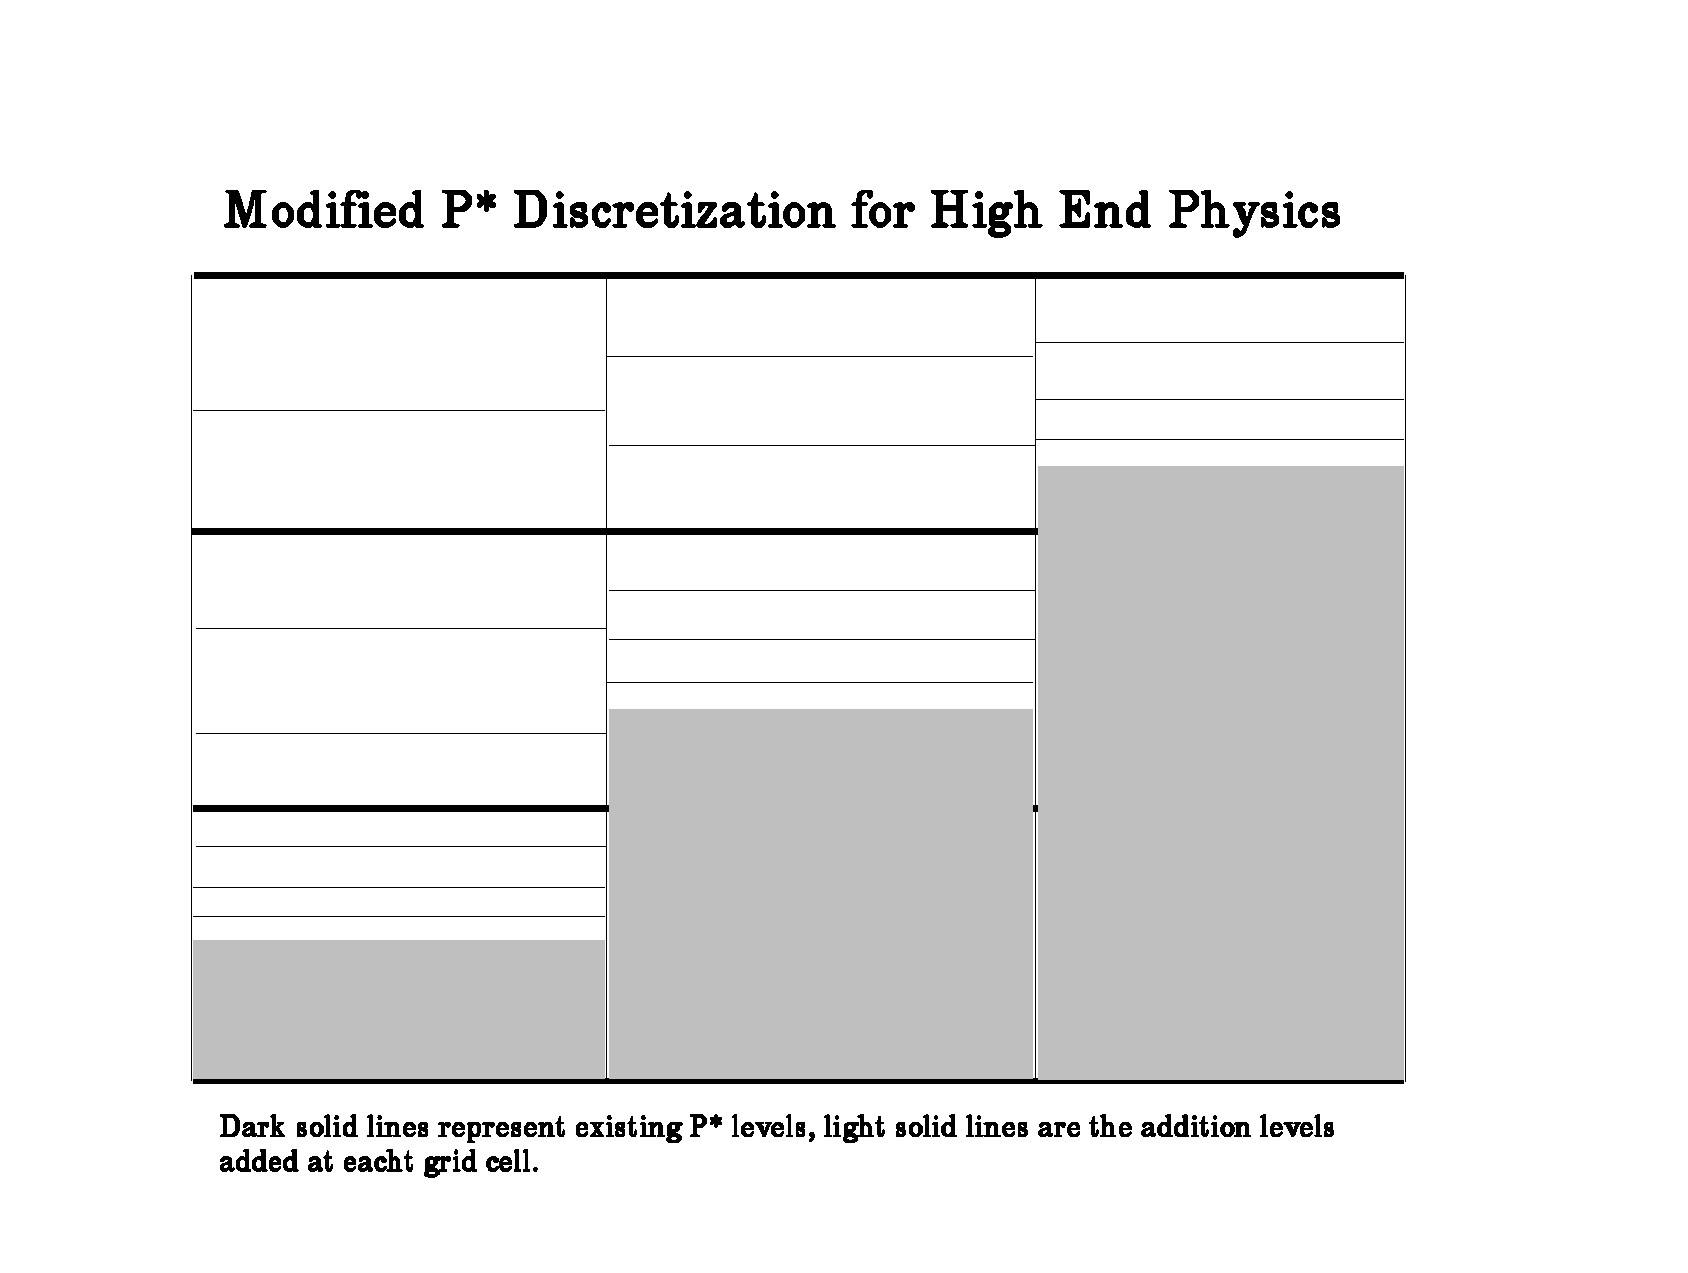
\includegraphics[height=2.4in]{part6/vertical.eps}
\caption{Vertical discretization for MITgcm (dark grey lines) and for the
atmospheric physics (light grey lines). In this implementation, all MITgcm level
interfaces must coincide with atmospheric physics level interfaces.}
\end{center}
\end{figure}

The algorithm presented here retains the state variables on the high resolution 'physics'
grid as well as on the coarser resolution 'dynamics` grid, and ensures that the two 
estimates of the state 'agree' on the coarse resolution grid.  It would have been possible 
to implement a technique in which the tendencies due to atmospheric physics are computed 
on the high resolution grid and the state variables are retained at low resolution only. 
This, however, for the case of the turbulence parameterization,  would mean that the 
turbulent kinetic energy source terms, and all the turbulence terms that are written 
in terms of gradients of the mean flow, cannot really be computed making use of the fine 
structure in the vertical. 

\subsubsection{Equations on Both Grids}

In addition to computing the physical forcing terms of the momentum, thermodynamic and humidity 
equations on the modified (higher resolution) grid, the higher resolution structure of the 
atmosphere (the boundary layer) is retained between physics calculations. This neccessitates
a second set of evolution equations for the atmospheric state variables on the modified grid. 
If the equation for the evolution of $U$ on $p^*$ can be expressed as:
\[
\left . {\partial U \over {\partial t}} \right |_{p^*}^{total} = 
\left . {\partial U \over {\partial t}} \right |_{p^*}^{dynamics} + 
\left . {\partial U \over {\partial t}} \right |_{p^*}^{physics}
\]
where the physics forcing terms on $p^*$ have been mapped from the modified grid, then an additional 
equation to govern the evolution of $U$ (for example) on the modified grid is written:
\[
\left . {\partial U \over {\partial t}} \right |_{p^{*m}}^{total} = 
\left . {\partial U \over {\partial t}} \right |_{p^{*m}}^{dynamics} + 
\left . {\partial U \over {\partial t}} \right |_{p^{*m}}^{physics} +
\gamma ({\left . U \right |_{p^*}} - {\left . U \right |_{p^{*m}}})
\]
where $p^{*m}$ refers to the modified higher resolution grid, and the dynamics forcing terms have 
been mapped from $p^*$ space.  The last term on the RHS is a relaxation term, meant to constrain
the state variables on the modified vertical grid to `track' the state variables on the $p^*$ grid 
on some time scale, governed by $\gamma$. In the present implementation, $\gamma = 1$, requiring
an immediate agreement between the two 'states'.

\subsubsection{Time stepping Sequence}
If we write $T_{phys}$ as the temperature (or any other state variable) on the high
resolution physics grid, and $T_{dyn}$ as the temperature on the coarse vertical resolution
dynamics grid, then:

\begin{enumerate}
%\itemsep{-0.05in}

\item{Compute the tendency due to physics processes.}

\item{Advance the physics state: ${{T^{n+1}}^{**}}_{phys}(l) = {T^n}_{phys}(l) + \delta T_{phys}$.}

\item{Interpolate the physics tendency to the dynamics grid, and advance the dynamics
state by physics and dynamics tendencies:
${T^{n+1}}_{dyn}(L) = {T^n}_{dyn}(L) + \delta T_{dyn}(L) + [\delta T _{phys}(l)](L)$.}

\item{Interpolate the dynamics tendency to the physics grid, and update the physics
grid due to dynamics tendencies: 
${{T^{n+1}}^*}_{phys}(l)$ = ${{T^{n+1}}^{**}}_{phys}(l) + {\delta T_{dyn}(L)}(l)$.}

\item{Apply correction term to physics state to account for divergence from dynamics state:
${T^{n+1}}_{phys}(l)$ = ${{T^{n+1}}^*}_{phys}(l) + \gamma \{  T_{dyn}(L) - [T_{phys}(l)](L) \}(l)$.} \\
Where $\gamma=1$ here. 

\end{enumerate}

\subsubsection{Interpolation}
In order to minimize the correction terms for the state variables on the alternative,
higher resolution grid, the vertical interpolation scheme must be constructed so that
a dynamics-to-physics interpolation can be exactly reversed with a physics-to-dynamics mapping.
The simple scheme employed to achieve this is:\\

Coarse to fine:\
For all physics layers l in dynamics layer L, $ T_{phys}(l) = \{T_{dyn}(L)\} = T_{dyn}(L) $.

Fine to coarse:\
For all physics layers l in dynamics layer L, $T_{dyn}(L) = [T_{phys}(l)] = \int{T_{phys} dp } $.\\

Where $\{\}$ is defined as the dynamics-to-physics operator and $[ ]$ is the physics-to-dynamics operator, $T$ stands for any state variable, and the subscripts $phys$ and $dyn$ stand for variables on
the physics and dynamics grids, respectively.

\subsubsection {Key subroutines, parameters and files } 

\noindent
One of the central elements of the gridalt package is the routine which 
is called from subroutine gridalt\_initialise to define the grid to be
used for the high end physics calculations. Routine make\_phys\_grid
passes back the parameters which define the grid, ultimately stored 
in the common block gridalt\_mapping.

\begin{verbatim}
       subroutine make_phys_grid(drF,hfacC,im1,im2,jm1,jm2,Nr,
     . Nsx,Nsy,i1,i2,j1,j2,bi,bj,Nrphys,Lbot,dpphys,numlevphys,nlperdyn)
c***********************************************************************
c Purpose: Define the grid that the will be used to run the high-end
c          atmospheric physics.
c
c Algorithm: Fit additional levels of some (~) known thickness in
c          between existing levels of the grid used for the dynamics
c
c Need:    Information about the dynamics grid vertical spacing
c
c Input:   drF         - delta r (p*) edge-to-edge
c          hfacC       - fraction of grid box above topography
c          im1, im2    - beginning and ending i - dimensions
c          jm1, jm2    - beginning and ending j - dimensions
c          Nr          - number of levels in dynamics grid
c          Nsx,Nsy     - number of processes in x and y direction
c          i1, i2      - beginning and ending i - index to fill
c          j1, j2      - beginning and ending j - index to fill
c          bi, bj      - x-dir and y-dir index of process
c          Nrphys      - number of levels in physics grid
c
c Output:  dpphys      - delta r (p*) edge-to-edge of physics grid
c          numlevphys  - number of levels used in the physics
c          nlperdyn    - physics level number atop each dynamics layer
c
c NOTES: 1) Pressure levs are built up from bottom, using p0, ps and dp:
c              p(i,j,k)=p(i,j,k-1) + dp(k)*ps(i,j)/p0(i,j)
c        2) Output dp's are aligned to fit EXACTLY between existing
c           levels of the dynamics vertical grid
c        3) IMPORTANT! This routine assumes the levels are numbered
c           from the bottom up, ie, level 1 is the surface.
c           IT WILL NOT WORK OTHERWISE!!!
c        4) This routine does NOT work for surface pressures less
c           (ie, above in the atmosphere) than about 350 mb
c***********************************************************************
\end{verbatim}

\noindent In the case of the grid used to compute the atmospheric physical
forcing (fizhi package), the locations of the grid points move in time with 
the MITgcm $p^*$ coordinate, and subroutine gridalt\_update is called during 
the run to update the locations of the grid points:

\begin{verbatim}
       subroutine gridalt_update(myThid)
c***********************************************************************
c Purpose: Update the pressure thicknesses of the layers of the
c          alternative vertical grid (used now for atmospheric physics).
c
c Calculate: dpphys    - new delta r (p*) edge-to-edge of physics grid
c                        using dpphys0 (initial value) and rstarfacC
c***********************************************************************
\end{verbatim}

\noindent The gridalt package also supplies utility routines which perform
the mappings from one grid to the other. These routines are called from the 
code which computes the fields on the alternative (fizhi) grid.

\begin{verbatim}
      subroutine dyn2phys(qdyn,pedyn,im1,im2,jm1,jm2,lmdyn,Nsx,Nsy,
     . idim1,idim2,jdim1,jdim2,bi,bj,windphy,pephy,Lbot,lmphy,nlperdyn,
     . flg,qphy)
C***********************************************************************
C Purpose:
C   To interpolate an arbitrary quantity from the 'dynamics' eta (pstar)
C               grid to the higher resolution physics grid
C Algorithm:
C   Routine works one layer (edge to edge pressure) at a time.
C   Dynamics -> Physics retains the dynamics layer mean value,
C   weights the field either with the profile of the physics grid
C   wind speed (for U and V fields), or uniformly (T and Q)
C
C Input:
C   qdyn..... [im,jm,lmdyn] Arbitrary Quantity on Input Grid
C   pedyn.... [im,jm,lmdyn+1] Pressures at bottom edges of input levels
C   im1,2 ... Limits for Longitude Dimension of Input
C   jm1,2 ... Limits for Latitude  Dimension of Input
C   lmdyn.... Vertical  Dimension of Input
C   Nsx...... Number of processes in x-direction
C   Nsy...... Number of processes in y-direction
C   idim1,2.. Beginning and ending i-values to calculate
C   jdim1,2.. Beginning and ending j-values to calculate
C   bi....... Index of process number in x-direction
C   bj....... Index of process number in x-direction
C   windphy.. [im,jm,lmphy] Magnitude of the wind on the output levels
C   pephy.... [im,jm,lmphy+1] Pressures at bottom edges of output levels
C   lmphy.... Vertical  Dimension of Output
C   nlperdyn. [im,jm,lmdyn] Highest Physics level in each dynamics level
C   flg...... Flag to indicate field type (0 for T or Q, 1 for U or V)
C
C Output:
C   qphy..... [im,jm,lmphy] Quantity at output grid (physics grid)
C
C Notes:
C   1) This algorithm assumes that the output (physics) grid levels
C      fit exactly into the input (dynamics) grid levels
C***********************************************************************
\end{verbatim}

\noindent And similarly, gridalt contains subroutine phys2dyn.

\subsubsection {Gridalt Diagnostics}
\label{sec:pkg:gridalt:diagnostics}

{\footnotesize
\begin{verbatim}

------------------------------------------------------------------------
<-Name->|Levs|<-parsing code->|<--  Units   -->|<- Tile (max=80c) 
------------------------------------------------------------------------
DPPHYS  | 20 |SM      ML      |Pascal          |Pressure Thickness of Layers on Fizhi Grid
\end{verbatim}
}

\subsubsection {Dos and donts}

\subsubsection {Gridalt Reference} 
